\section{Critical Path Method in practice}
Primary a network plan delivers a time economic planning of a sequence of tasks. In addition , it also provides an excellent mean for flow control. For example you have the possibility to check whether a task is solved or it is open. Moreover you can avoid critical path. Therefore, a Critical Path Method network plan is a good opportunity to manage projects. If you think about a project then two kinds of projects come into your mind. On the one hand small projects, which can be handled manually and on the other hand there are big projects, which would be a real challenge to handle manually. Therefore it is necessary to use software solutions, that make the work more convenient and efficient. 

For this reason this chapter would focus on “Critical Path Method” in practice. At first we would focus on simple Critical Path Method calculation which can be done with simple spreadsheet applications. We will demonstrate this in a small OpenOffice example. Moreover this is a good approach to illustrate how “Critical Path Method” works.
In a further step we would focus on “real” Critical Path Method tools. On the one hand we would give an overview over MS Project, which is the Microsoft's commercial approach of a project planning software. And we would also demonstrate “OpenProj” which is an open source approach of an project management application. Afterwards we would compare them and give a listing with a lot of other useful project management software.

Finally we would finish this chapter with a conclusion part.

\subsection{Spreadsheet Applications}
Spreadsheet Applications are common tools, which can be used by nearly every user. Most of the computer users have such an application installed on their operating system. For example the commercial program Microsoft Excel or the open source program Open Office are such spreadsheet applications. In this chapter we would illustrate the critical path method with Open Office Calculator. Moreover it is a good way to realize how the calculation of the critical path works.

At first we must draw a precedence graph that describes the flow of project activities. For example Figure \ref{pic:seqChart}  illustrates such a graph. 

\begin{figure}[h] 
\centerline{\fbox{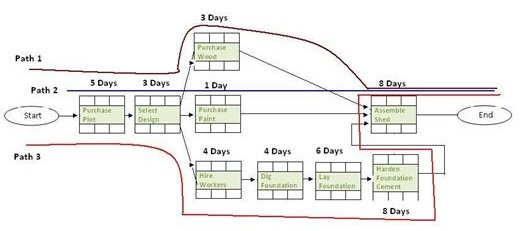
\includegraphics[width=100mm]{CPM_graph}}}
\caption{Precedence graph}
\label{pic:seqChart}
\end{figure}

For the Calculation of the Critical Path we used OpenOffice 3.0.1. 
In a second step we have to define the activities and the duration in the spreadsheet. Such activities can be project milestones, for example purchase a plot and selecting a design. Moreover these project steps have values, we call these values duration. For example typical values for duration are hours, days or months. We get these activities and their duration from the precedence graph. If we have them we can enter them in our spreadsheet. We take for every activity and the corresponding duration one table column.

At this point we must identify the paths in the precedence graph. If the path contains a activity we insert a one into our spreadsheet otherwise we insert a zero. Otherwise means that the activity isn't contained in the path.  We can easily realize this in our spreadsheet, for example we use for every path a new row and in every “activity” column we insert the corresponding values (one or zero). 

Afterwards we calculate the path duration. Therefore we must add up the duration of all the identified activities of a path. If we have the duration of each path we must calculate the maximum path duration. In other words this is the longest path in our precedence graph.

In a last step we must compare all the path durations with the longest path. If there is a path duration that is equal to the longest path duration, we have identified a critical path.
 
All these described things are illustrated in figure \ref{pic:office}. Moreover it is to mention that the demonstration in figure \ref{pic:office} uses the precedence graph of figure \ref{pic:seqChart}.
\begin{figure}[h] 
\centerline{\fbox{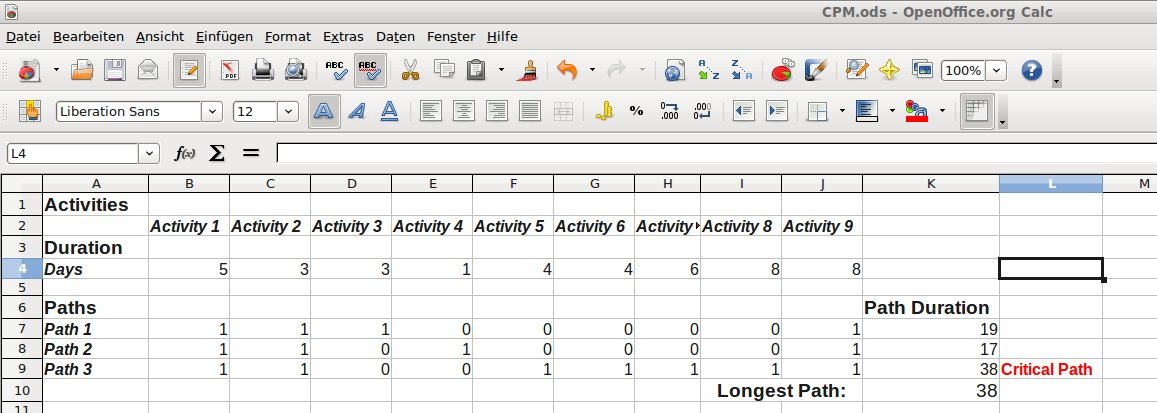
\includegraphics[width=150mm]{CPM_office}}}
\caption{CPM calculation in OpenOffice}
\label{pic:office}
\end{figure}


After we have identified the critical path we can create a project schedule which avoids critical path. Finally, it is to mention that this can be also done with Microsoft Excel. Maybe some simple modifications of the algorithm must be done, because Microsoft Excel and OpenOffice differ in some points.

\subsection{Critical Path features in project Management software}
We have seen that it is possible to calculate the Critical Path with spreadsheet applications. It is a good way to demonstrate the critical path method, but it isn't a comfortable way to identify it. If we think of a project that has more than 100 activities and a lot of paths, it would take a lot of time to calculate the critical path with OpenOffice or Microsoft Excel. 

For this reason we must look for software solutions that can calculate the critical path in large projects. There are a lot of diverse project management software solutions on the market which can solve this task. We would demonstrate two of them, on the one hand we would present some facts about Microsoft Project, which is an commercial product and very famous. This software program has a lot of competitors and for this reason we want to introduce one of them, the so called program OpenProj. It is an open source approach of a project management software. Afterwards we would give an comparison between the commercial and the open source approach of a project management software.

Finally we would show a list with alternative project managementsoftware.

\subsubsection{Microsoft Project}
Microsoft Project (=MS Project) is a project management software, it is made to plan, control and manage large projects. Moreover it should alleviate the management tasks of a project manager. 
The Software has been developed by Microsoft and there are a lot of diverse versions on the market. The latest Version is Microsoft Project 2010. The software is a commercial approach of an project management software.
The applications gives to the users the possibility to create critical path schedules, critical chain and event chains methodologies. Moreover a lot of add-ons exist, that make the work with the software more convenient. Moreover the software cannot be used only by the project manager, also employees have access to it and can for example see the project schedule or workload for the project.

Microsoft Project delivers the following core features:
\begin{enumerate}
\item Effective Work Planning:
\item Effective Resource Management
\item Efficient Communication and Collaboration
\item Quick Access to Information
\item Effective Leveraging of Existing Data
\end{enumerate}

At his point we won't go into detail of all the features, because this would go beyond the scope of the paper.

The “Effective Work Planning” is very important in our context. The critical path method is used to support the creation of a project schedule. 
If we want to create a project schedule we must have activities or tasks and we must know the duration of them, if we have specified them then we can generate a Gantt Chart. Then we can insert this data via an user interface to the software In some sense this task is comparable to what we have done with spreadsheet applications. These things are illustrated in figure \ref{pic:msproject}.

\begin{figure}[h!!] 
\centerline{\fbox{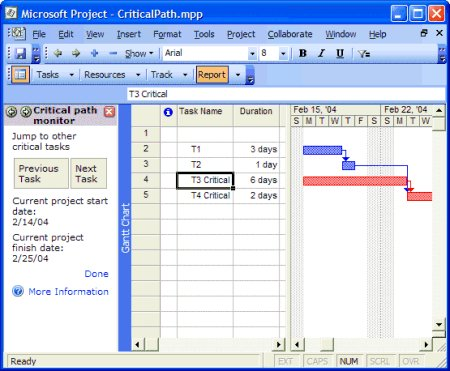
\includegraphics[width=65mm]{CPM_msproject}}}
\caption{Screenshot Microsoft Project}
\label{pic:msproject}
\end{figure}

As you can see in figure 3 it is very convenient to create a project schedule wit MS Project. The critical path is indicated with a red chart. Moreover there a lot of other useful features and for this reason this project management software is very popular.

\subsubsection{OpenProj}
OpenProj is an open source project management software and it is very similar to the commercial product Microsoft Office. Moreover it is written in Java and therefore it is portable to a lot of different platforms. For example you can run the program on a Mac Operating System, windows operating System or unix based operating system.
The software has been developed by Serena Software and the latest Version is OpenProj 1.4.

As mentioned above, it is quite similar to Microsoft Office. The software is used to plan, manage and control a project.

OpenProj delivers the following core features:
\begin{enumerate}
\item Earned value costing
\item Gantt chart
\item PERT graph
\item Resource Breakdown Structure
\item Task usage Reports
\item Work Breakdown Structure
\end{enumerate}

We won't focus on the features in detail, but it is to mention that the critical path method is used in the Gantt charts for creating a project schedule. Moreover we must define activities and durations to generate a project schedule. Figure 4 shows a picture of the OpenProj project management software.

\begin{figure}[h!!] 
\centerline{\fbox{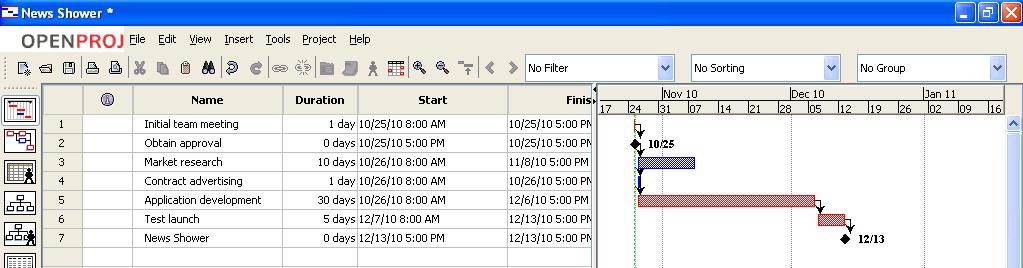
\includegraphics[width=150mm]{CPM_openproj}}}
\caption{Screenshot OpenProj}
\label{pic:openproj}
\end{figure}

The red chart in figure \ref{pic:openproj} shows a critical path. Moreover OpenProj has a lot other features for project management.
\subsubsection{Comparison of Microsoft Office and OpenProj}
In this chapter we have introduced Microsoft Office and OpenProj. Both of them are really powerful project management tools. For this reason we want to compare them to see the advantages of using them.

As mentioned before one big difference between them is, that Microsoft Office is commercial and therefore proprietary and OpenProj is free and open source. Therefore you have the possibility to change the source or add some features.
Moreover this leads us to the issue of  portability of the software. Microsoft Project is designed for Windows operating system and OpenProj is implemented in Java and therefore it can run on every operating system.

If we look at the performance of both of them we will see that OpenProj is a lightweight. In this context this means that OpenProj takes less computer resources to install than Microsoft Project.

If we look at the look and feel, we will discover, that the look quite similar. One big advantage of Microsoft Project is, that they have a Help documentation, which is very useful to learn interacting with the software. Furthermore this documentation is online and offline available.

Another big advantage is that Microsoft Project is compatible with all Microsoft Office file formats, which is very important, because a lot of people or companies use them. Moreover these files can be imported into Microsoft Project.

Finally it is to mention that both of them provide the following features and functions:
\begin{itemize}
\item Gantt charts
\item A project Network
\item Resource Charts
\item Work Breakdown Structure
\item Resource Breakdown Structure
\end{itemize}
\subsubsection{List of alternative project Management Software}
There exist a lot of other project management software. The following list gives an overview about them.

Alternative project management software:
\begin{itemize}
\item Clarizan
\item DynaRoad
\item OmniPlan
\item Project.net
\item Primavera
\item Planta Project
\item Open Workbench
\item Ganttprojact
\end{itemize}

\subsection{Conclusion} 
This chapter showed the practical use of the critical path method in project management software. We saw two approaches of calculating the critical path. On the one hand we saw how we can do the calculation with a simple spreadsheet application and on the other hand we saw how we can use software for larger projects. Besides, we saw that it is more convenient and efficient to use a project management software as Microsoft Office to get the critical path. Finally, it is to mentioned that the critical path method is only one simple function of these kind of software. Furthermore you can find the critical path method in a lot of other applications and programs.

